\section{W06 - Supply Management \& Distribution}
\subsection{Supplier Network Configuration}
\subsubsection{Case Study: Dell}
\subsubsection{Market Shares until 2000}
\subsubsection{Market Shares until 2006}
\subsubsection{Market Shares today}
\subsubsection{Comparing Operating Margins}
\subsubsection{Dell's Supply Network}
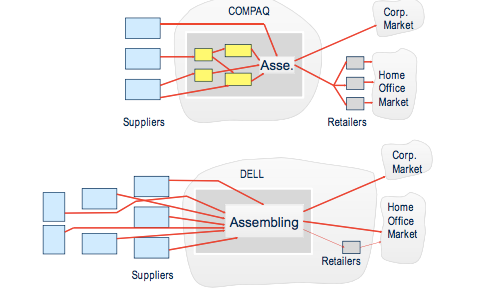
\includegraphics[width=1\textwidth]{W06/dellssupplynetwork}
\subsubsection{Dell's Innovative Financing Model: Another Factor in Its Success}
\subsubsection{PC Design Evolution}
\subsubsection{Structure of Supply Networks\index{Supply!Networks}}
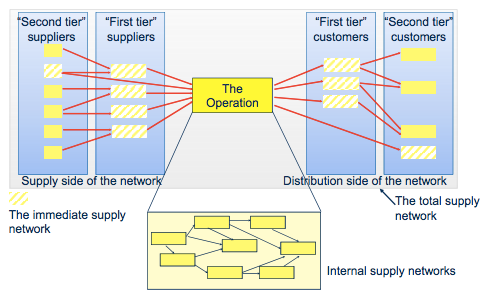
\includegraphics[width=1\textwidth]{W06/structureofsupplynetwork}	
\subsubsection{OperationsPerformance\index{Operations!Performance}: A Whole Supply Chain \index{Supply!Chain}Issue}
Benefits of looking at the whole supply chain include:
\begin{itemize}
	\item It puts the operation into its competitive context
	\item It helps to identify the keay players
	\item It shifts emphasis to the long term
	item It sensitizes the operation to macro-changes
\end{itemize}
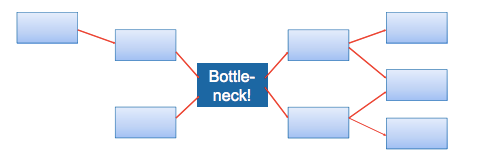
\includegraphics[width=1\textwidth]{W06/supplychainissue}	
\subsubsection{Supply Network\index{Supply!Network} Design: Extension of Process Span}
Example for horizontal integration: google into car production (not in the own supply chain). \\ \index{Integration!horizontal} \index{Upstream!vertical Integration}
\index{Downstream!vertical Integration}
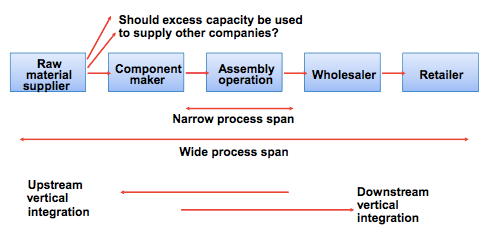
\includegraphics[width=1\textwidth]{W06/extensionofprocessspan}	
\subsubsection{The Decision Logic of Outsourcing\index{Outsourcing}}
Know How strategisch -> kein Outsourcing
Outsourcing nur aus Kostengr\"unden ist nicht Lohnenswert.\\
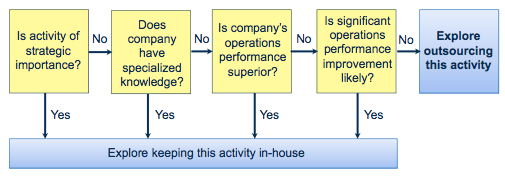
\includegraphics[width=1\textwidth]{W06/outsourcing1}
\subsubsection{Relationship between Offshoring\index{Offshoring} and Outsourcing\index{Outsourcing}}
\begin{center}
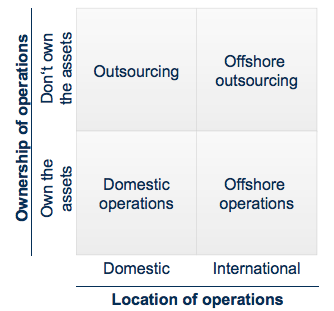
\includegraphics[width=0.5\textwidth]{W06/outsourcingvsoffshoring}
\end{center}

\subsubsection{Trends in Outsourcing\index{Outsourcing} Example: Automotive Industry}
Percentage of in-house value creation of German automotive OEM\index{OEM}s - Wertsch\"opfung = Kosten + Marge? \\
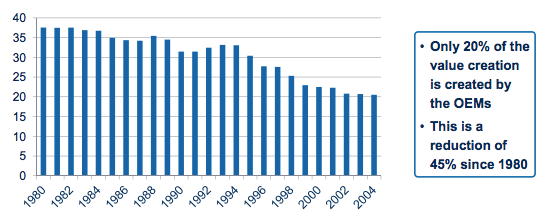
\includegraphics[width=1\textwidth]{W06/autooem}
\subsection{Supplier Management}
\subsubsection{The complexity of \index{Supplier Management} forces an systematic approach – Example Metro Germany}
\subsubsection{A material classificaiton is the basis for a segmented approach towards suppliers}
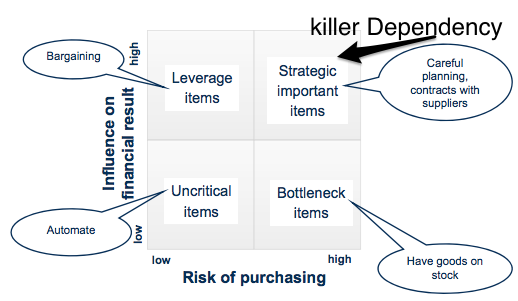
\includegraphics[width=1\textwidth]{W06/classification}
\subsubsection{How to segment your supplier – Example scorecard}
\subsubsection{Supplier Management\index{Supplier Management}: Measure and score their performanceregularly}
\subsubsection{An ambitious route of managing suppliers: Develop them further – example Toyota}
\subsection{Distribution\index{Distribution}}
\subsubsection{Distribution\index{Distribution}: From the Manufacturer to the Stores}
\subsubsection{Distribution\index{Distribution} and Channels\index{Channels}}
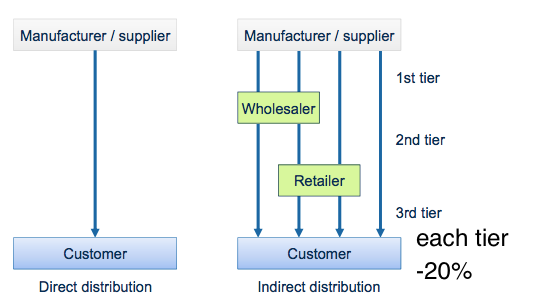
\includegraphics[width=1\textwidth]{W06/distributionandchannels}
\subsubsection{Transportation of Materials: Key Figures for Switzerland}
\subsubsection{Distribution: Example of Swiss Retailer}
\subsubsection{Cross-Docking\index{Cross-Docking}: Modern Distribution\index{Distribution} System}
Nichts mehr einlagern, nur kurz zwischenlagern, fixer \& schneller. Verteilzentren werden aufgel\"ost.\\
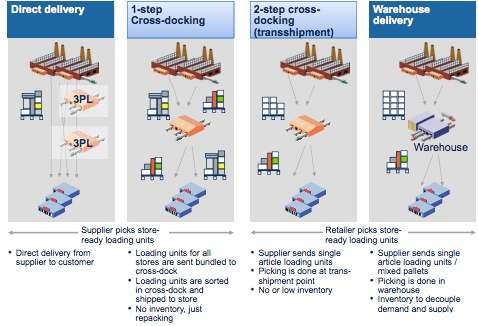
\includegraphics[width=1\textwidth]{W06/crossdocking}
\subsubsection{Indirect distribution costs are often overlooked}
3) zu viel an Lager\\
6) zu wenig an Lager\\
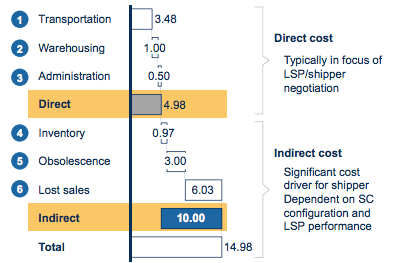
\includegraphics[width=1\textwidth]{W06/indirectcosts}